Neste apêndice apresentar-se-ão versões intermediárias do motor foguete desenvolvido, de modo a esclarecer algumas decisões tomadas ao longo do trabalho.

\begin{minipage}{.49\textwidth}
    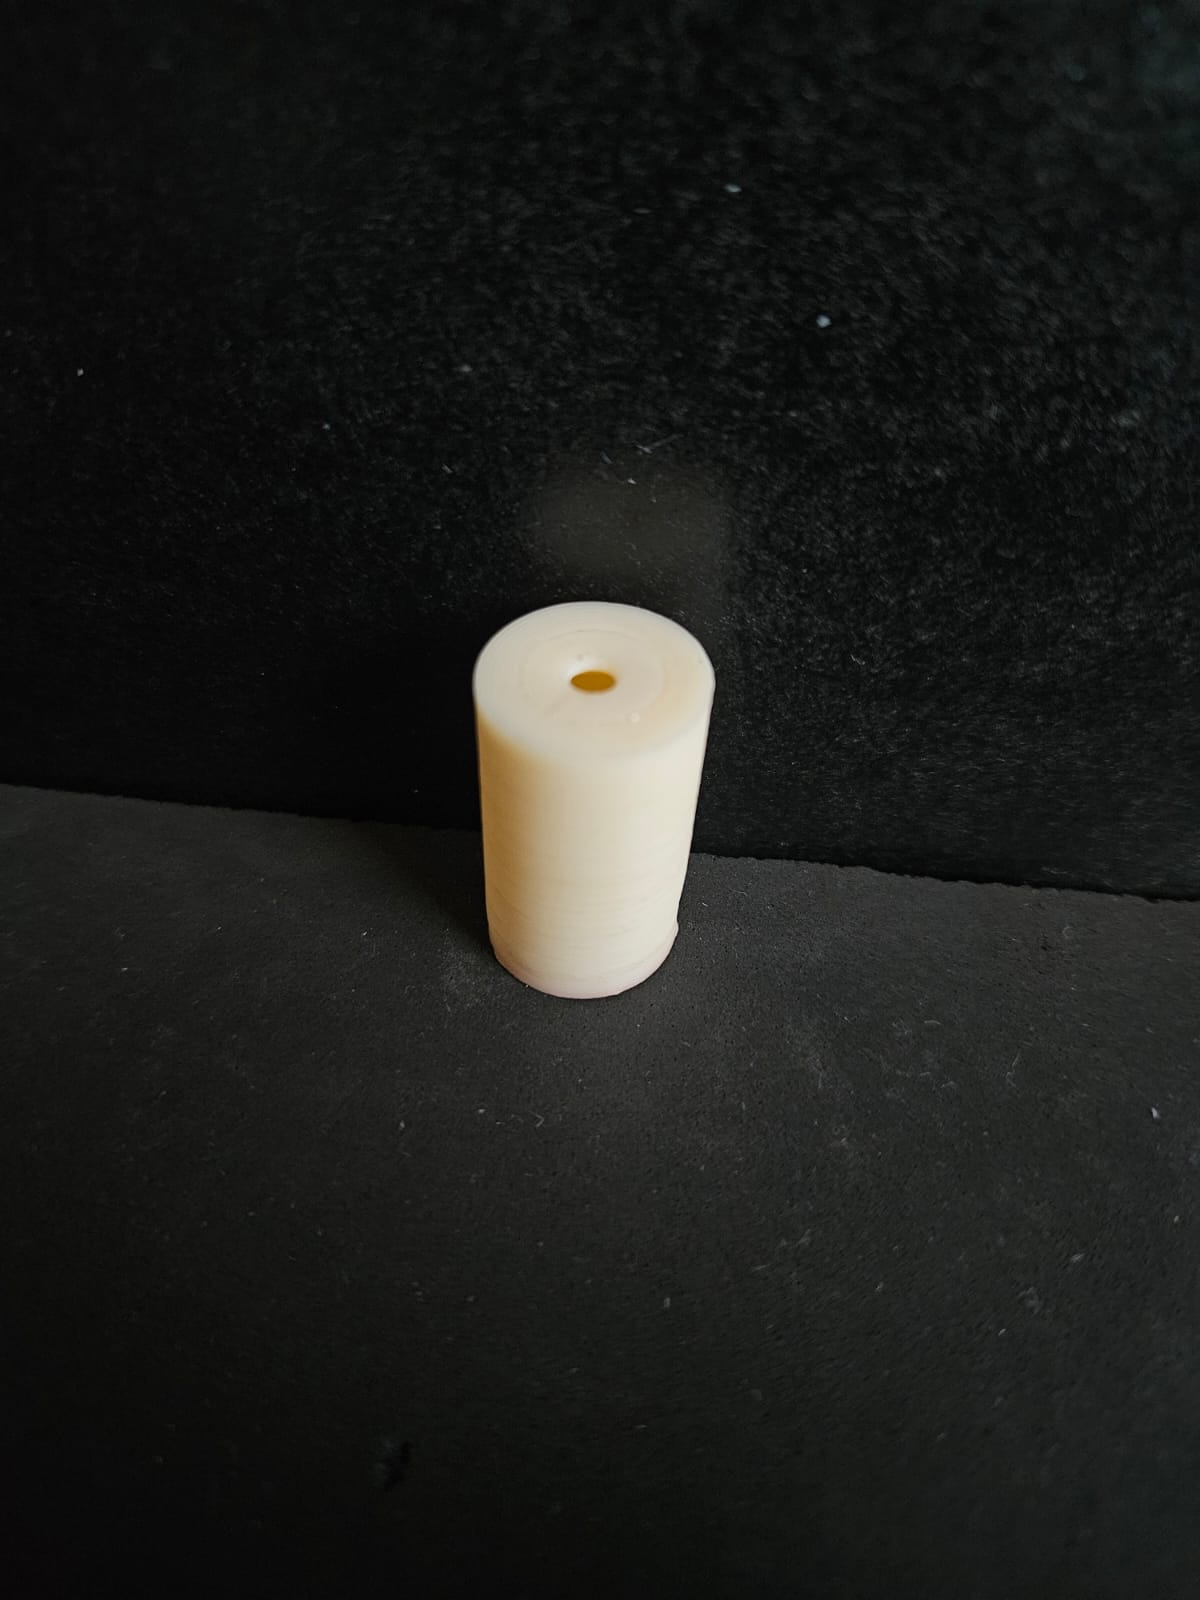
\includegraphics[width=\textwidth]{img/app_dev_history/motor1.jpeg}
\end{minipage}
\begin{minipage}{.49\textwidth}
    Primeiro motor desenvolvido. Apenas uma câmara cilíndrica com uma tubeira em uma base e um furo roscado para a mangueira de gás na outra. Projetado para \(F = 5\,\mathrm{N}\), \(p_c = 5\,\mathrm{bar}\), \(\alpha_{\mathrm{div}} = 15\,\mathrm{^\circ}\), \(\alpha_{\mathrm{conv}} = 45\,\mathrm{^\circ}\) e razão de contração 6. Provou-se de difícil manuseio e a tubeira foi impressa em poucas camadas, de modo que sua precisão dimensional foi subótima.
\end{minipage}

\begin{minipage}{.49\textwidth}
    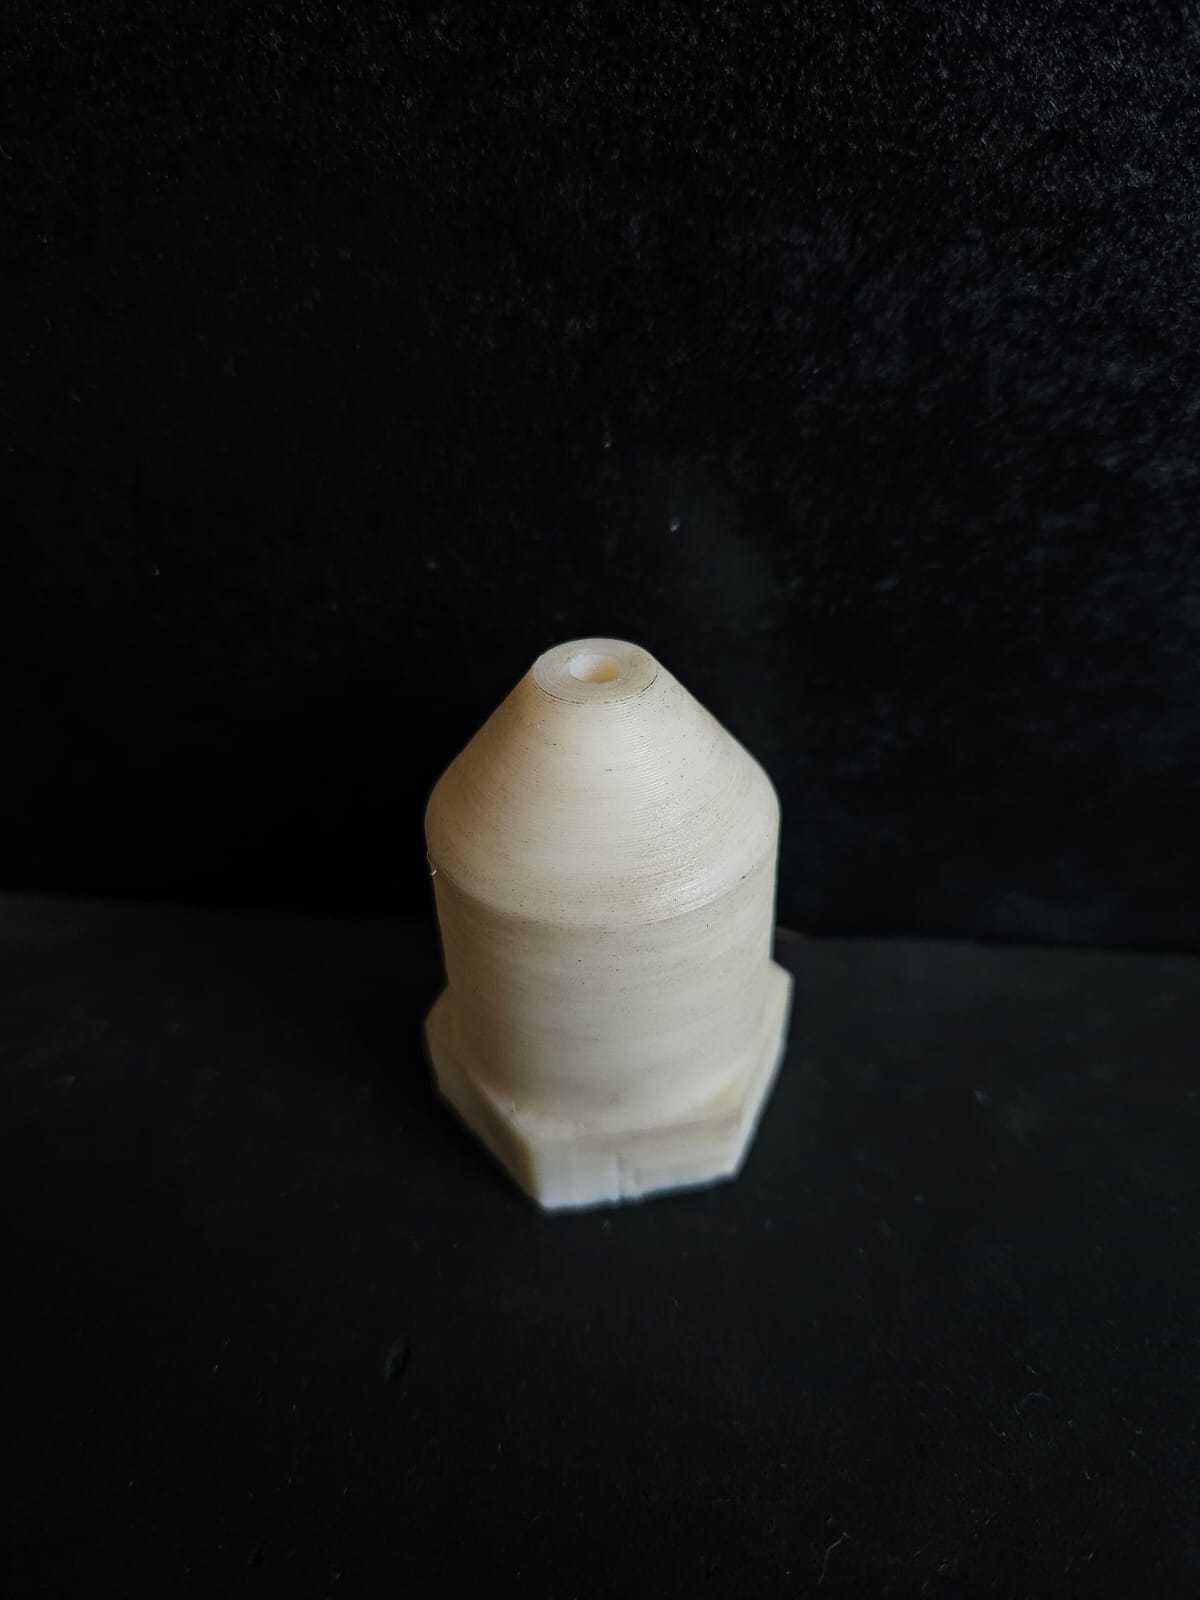
\includegraphics[width=\textwidth]{img/app_dev_history/motor2.jpeg}
\end{minipage}
\begin{minipage}{.49\textwidth}
    A razão de contração foi aumentada para 50, alongou-se a tubeira usando \(\alpha_{\mathrm{div}} = 15\,\mathrm{^\circ}\), a câmara foi alongada e foram adicionadas superfícies planas à base para facilitar o rosqueamento do conector de gás (base inferior, não visível na imagem). A cor encardida deve-se ao uso de cola de ABS para selar a peça, que apresentou grandes vazamentos de ar em testes preliminares.
\end{minipage}

\begin{minipage}{.49\textwidth}
    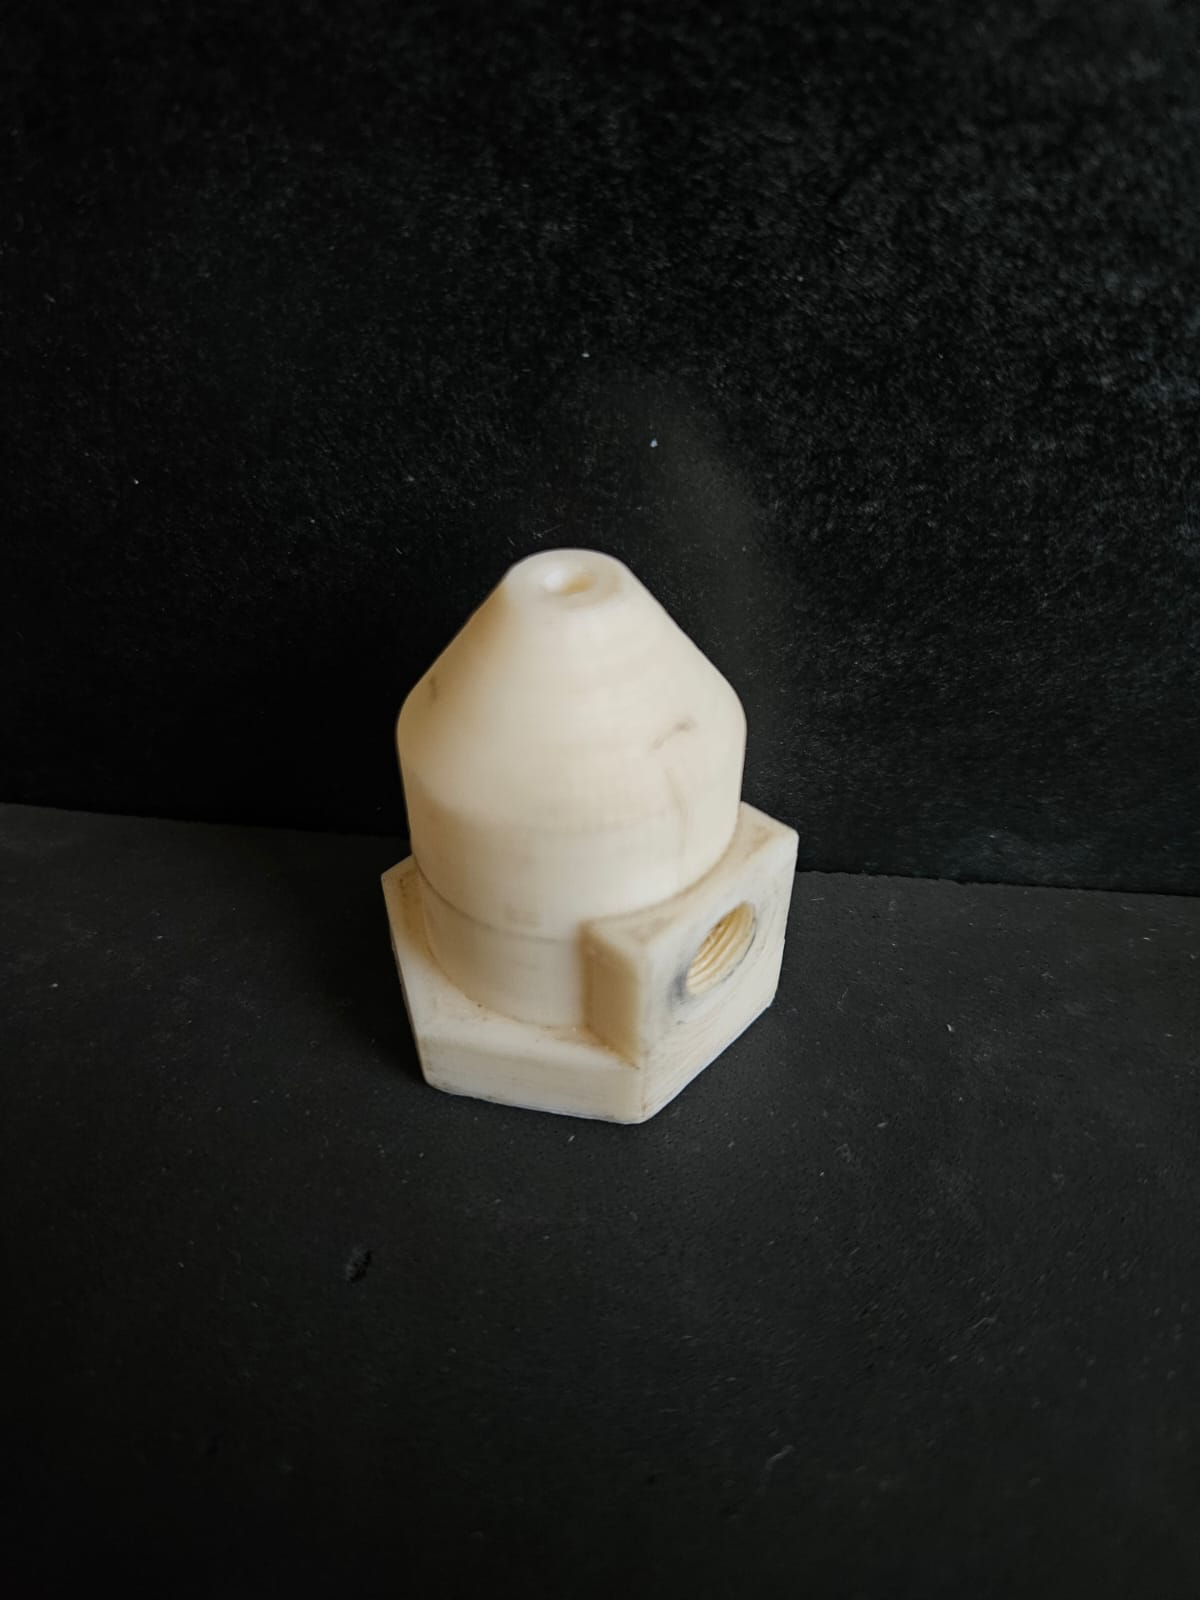
\includegraphics[width=\textwidth]{img/app_dev_history/motor3.jpeg}
\end{minipage}
\begin{minipage}{.49\textwidth}
    Adicionada entrada para conexão com um transdutor de pressão, ver seção~\ref{sec:method_validation}. O transdutor de pressão foi posicionado perpendicularmente à entrada de ar, na mesma posição da versão anterior, para medir a pressão estática na câmara.
\end{minipage}

\begin{minipage}{.49\textwidth}
    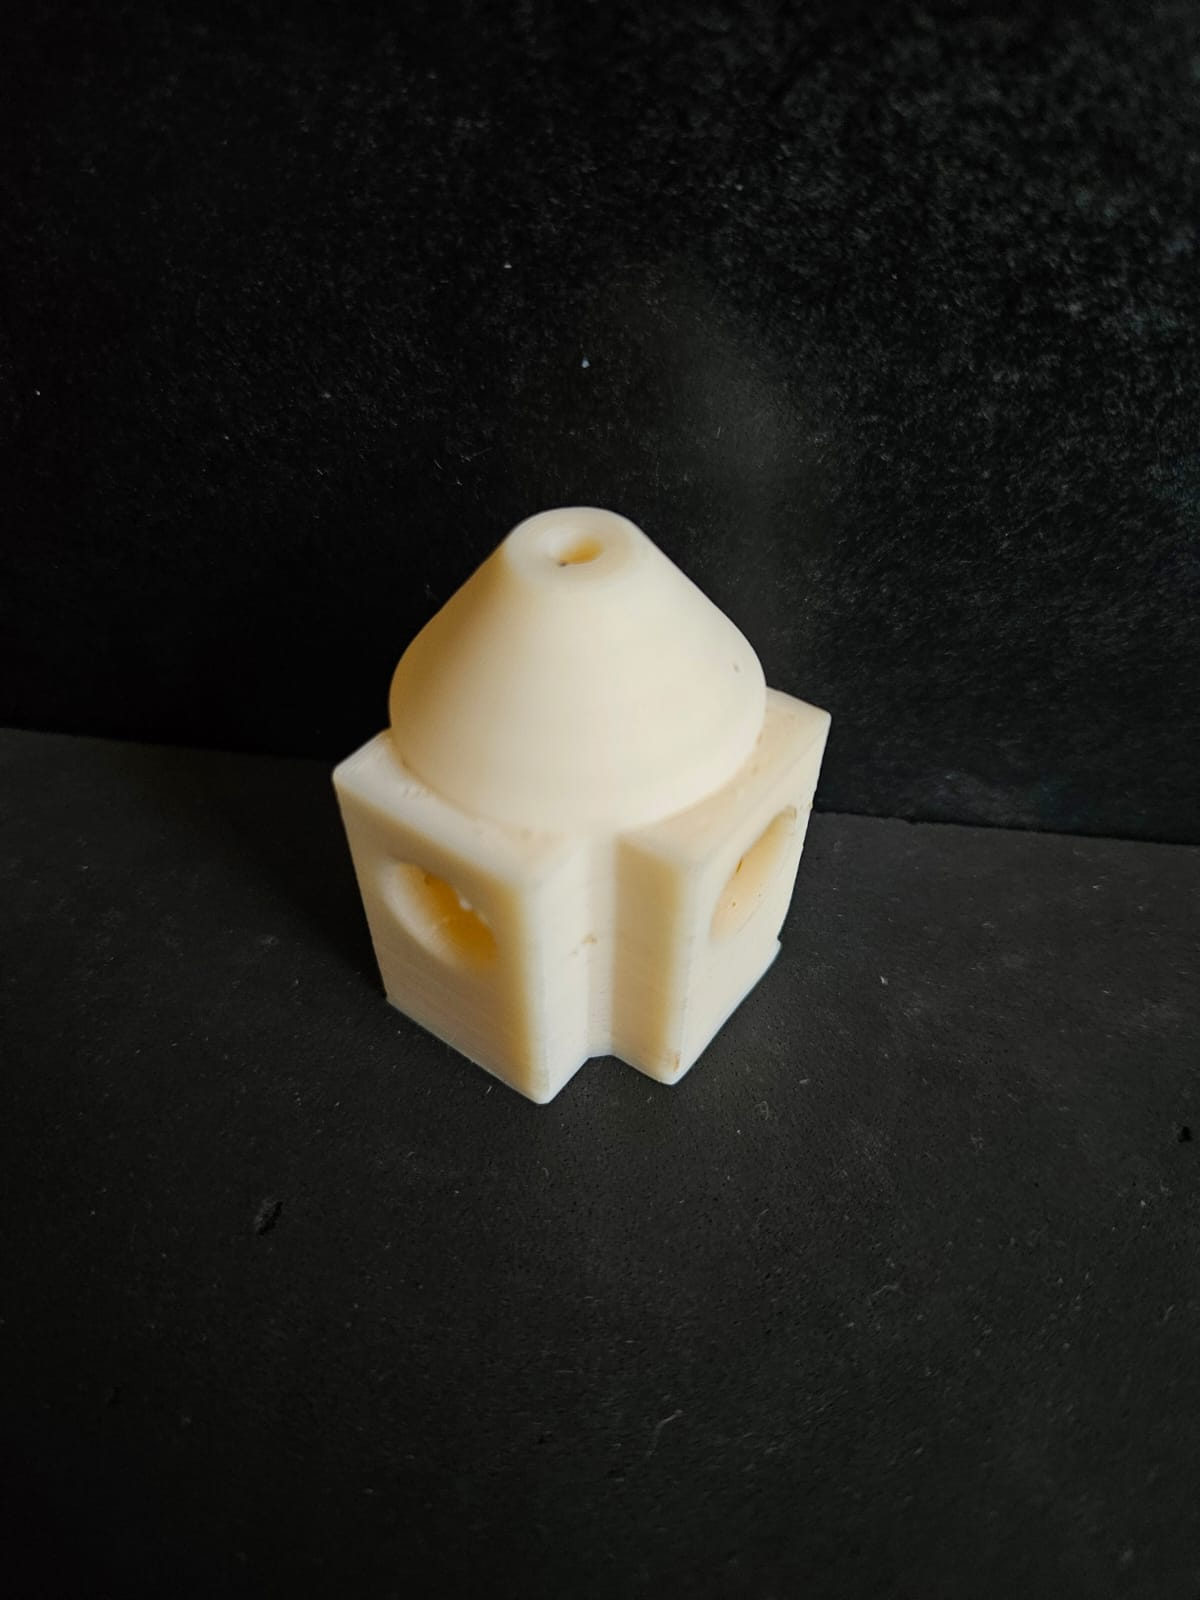
\includegraphics[width=\textwidth]{img/app_dev_history/motor4.jpeg}
\end{minipage}
\begin{minipage}{.49\textwidth}
    Ambas as conexões de gás agora são posicionadas em paredes laterais, e a geometria dos planos laterais foi mudada para quadrada, ao invés de hexagonal. A entrada de ar na base do motor dificultava sua montagem na bancada de teste de empuxo. O diâmetro das conexões de gás foi aumentado para reduzir perdas viscosas na tubulação, que estimavam-se ser altas devido à alta vazão.
\end{minipage}

\begin{minipage}{.49\textwidth}
    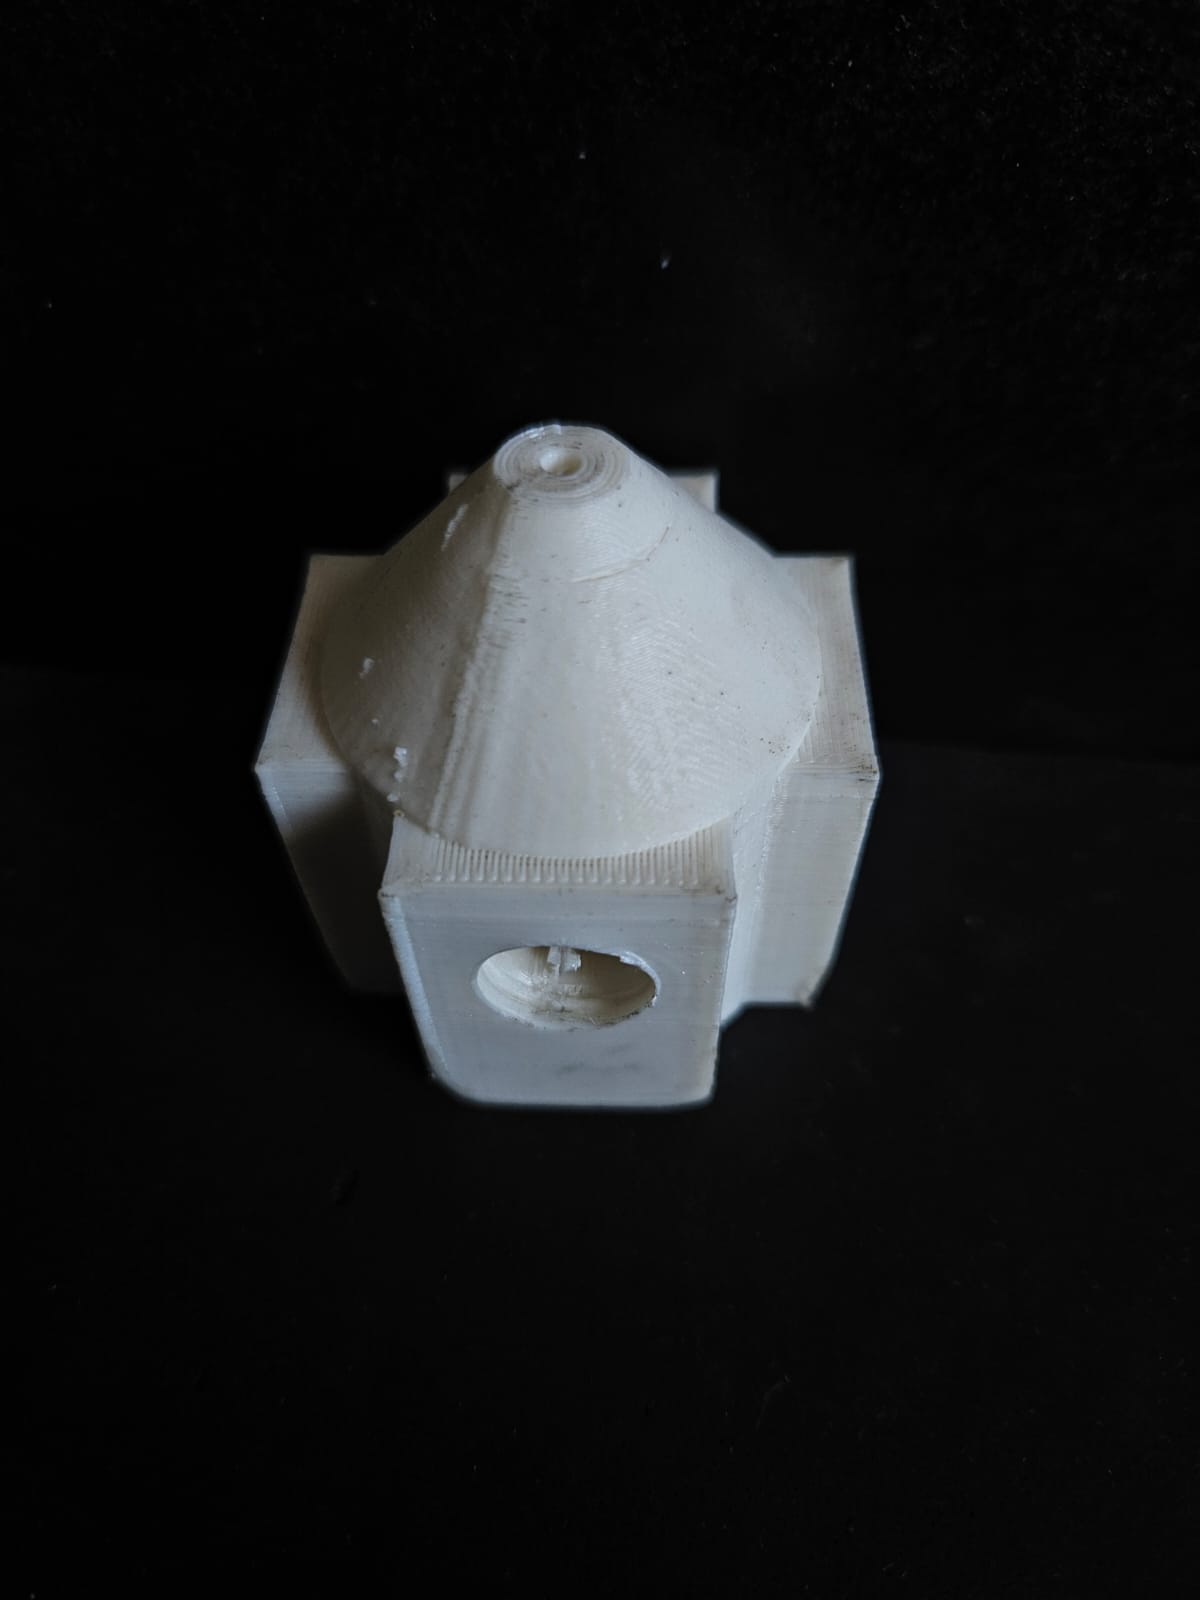
\includegraphics[width=\textwidth]{img/app_dev_history/motor5.jpeg}
\end{minipage}
\begin{minipage}{.49\textwidth}
    O empuxo do motor foi reduzido para \(2\,\mathrm{N}\). Neste ponto do trabalho, já havia-se testado os motores anteriores e foi consumida metade de um cilindro de nitrogênio comprimido. Visando reduzir custos e permitir testes mais extensivos, o empuxo foi reduzido para permitir o uso do compressor de baixa capacidade mencionado na~\ref{sec:discussion}. O extrusor usado a partir desse motor foi de \(0,2\,\mathrm{mm}\), ao invés de \(0,4\,\mathrm{mm}\) como nos motores anteriores, o que garantir maior precisão para a tubeira mais estreita. 
\end{minipage}

\begin{minipage}{.49\textwidth}
    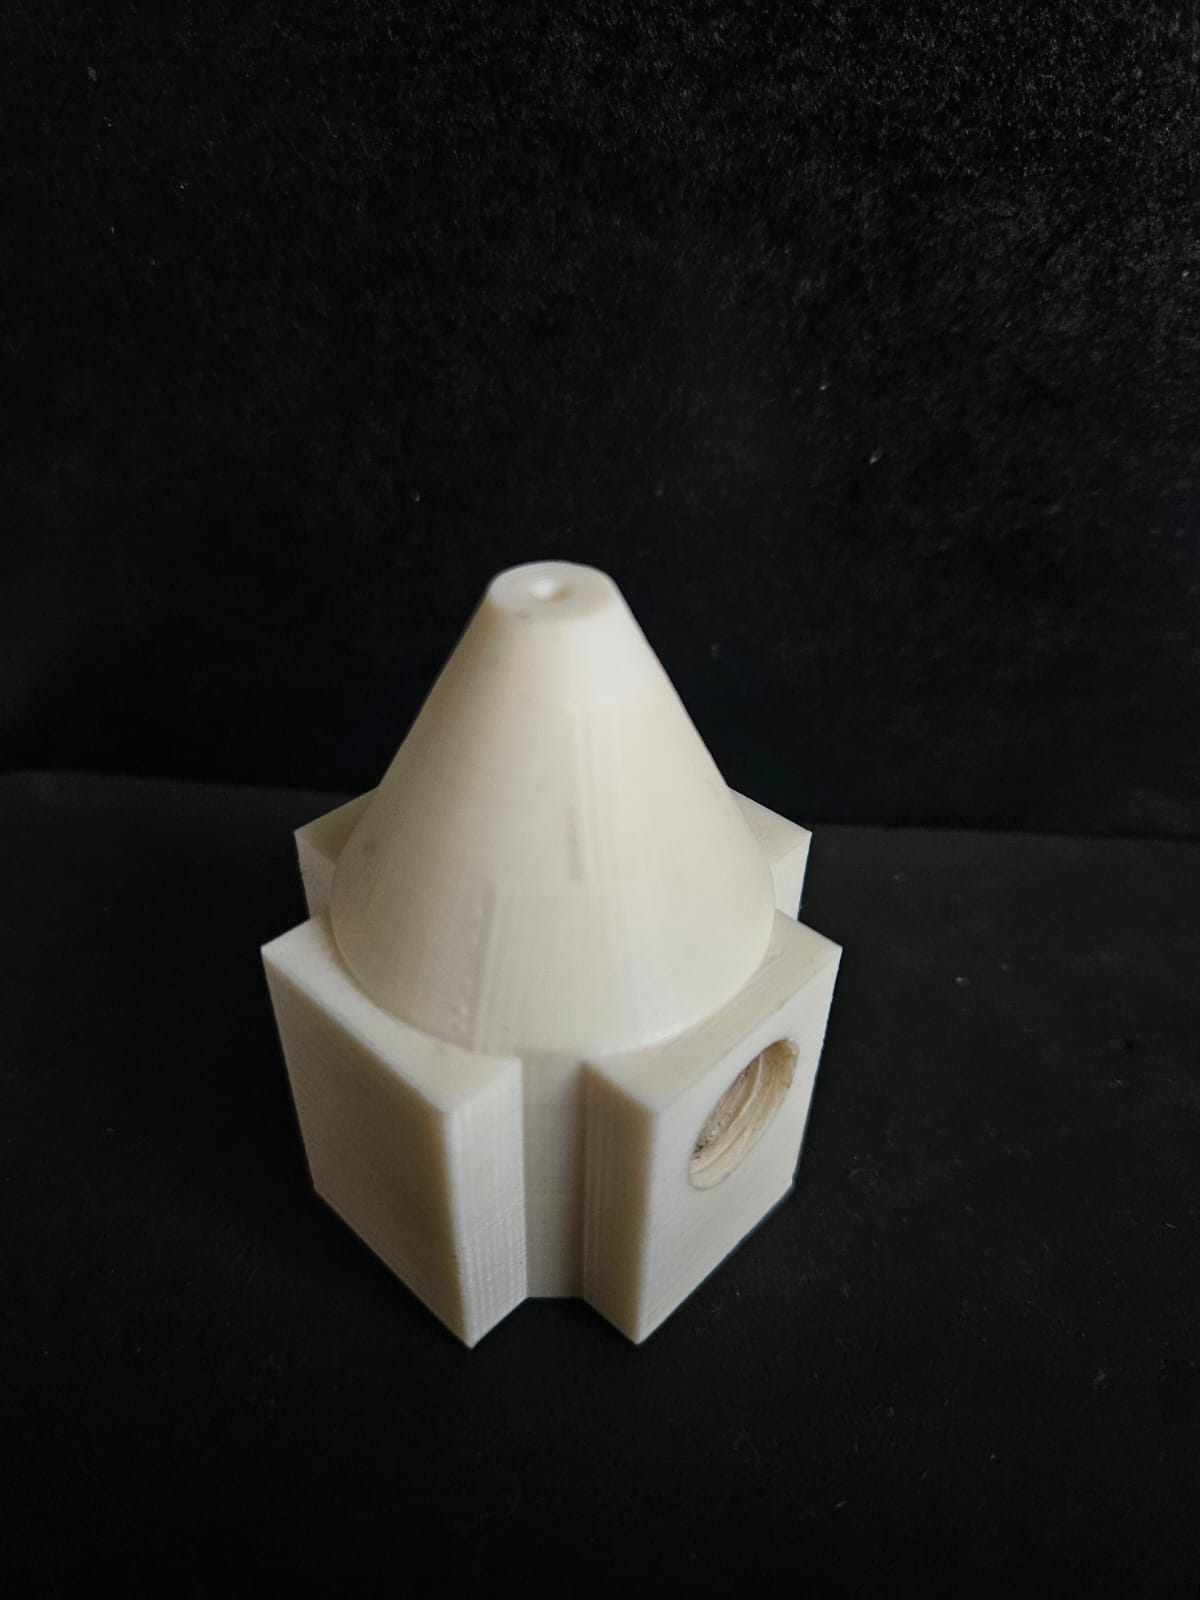
\includegraphics[width=\textwidth]{img/app_dev_history/motor6.jpeg}
\end{minipage}
\begin{minipage}{.49\textwidth}
    Versão final do motor. Alongou-se o conjunto, reduzindo o ângulo de convergente para \(\alpha_{\mathrm{conv}} = 30\,\mathrm{^\circ}\) para reduzir a distância da tubeira à lâmina defletora. 
\end{minipage}